\documentclass[10pt]{exam}
\usepackage[hon]{template-for-exam}
\usepackage{tikz,my-tikz-clipart}
\usetikzlibrary{shadings,decorations.pathmorphing,arrows.meta}


\title{Conservation of Energy Problems}
\author{Rohrbach}
\date{\today}

\begin{document}
\maketitle

\section*{Consolidation}

A rollercoaster ($m = 1000$ kg) starts from rest at the top of a 50 m hill.  The tracks are frictionless.

\vspace{1em}


\begin{parts}
  \part
    If the hill goes all the way down to the ground, how fast should it be going at that point?
  \part
    Next, the rollercoaster continues to the top of the next hill, which is 35 m high.  What is its velocity at the top of the next hill?
\end{parts}

\vspace{1em}

    
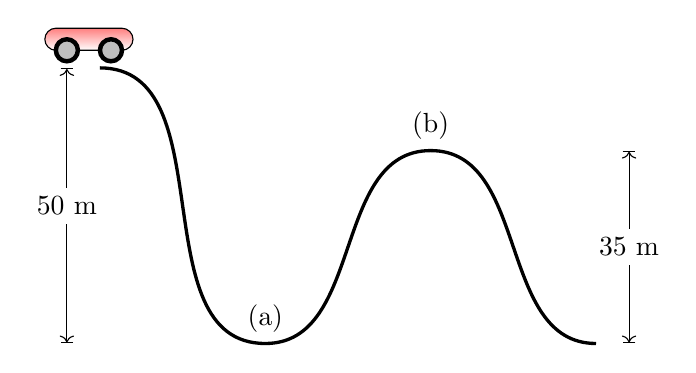
\begin{tikzpicture}[x=0.7cm, y=0.7cm]
  \def\xs{3}
  \draw[very thick] 
    (1*\xs,5) 
    to[in=180,out=0] (2*\xs,0) node[above] {(a)}
    to[in=180,out=0] (3*\xs,3.5) node[above] {(b)}
    to[in=180,out=0] (4*\xs,0);

  \draw[|<->|] (.8*\xs,0) -- (.8*\xs,5) 
    node[midway,fill=white] {50 m};
  \draw[|<->|] (4.2*\xs,0) -- (4.2*\xs,3.5) 
    node[midway,fill=white] {35 m};


  \begin{scope}[scale=0.4,shift={(5,13.3)}]
    \filldraw[top color=red!50, draw=black, rounded corners] 
      (0,0) -- (0,1) -- 
      (4,1) -- (4,0) -- cycle;
    \draw[fill=gray!50, draw=black, ultra thick] 
      (1,0) circle (.5);
    \draw[fill=gray!50, draw=black, ultra thick] 
      (3,0) circle (.5);
  \end{scope}

\end{tikzpicture}



\pagebreak

\section*{Practice Problems}

\begin{questions}
  \question

  A spring of constant $k= 200$~N/m is used in the launcher of a pinball machine. The player pulls back on the knob, so the spring is compressed by 0.15~m from its equilibrium position by a pinball of mass 0.13 kg. When the spring is released, the ball is shot forward (it is not attached to the spring). After release the ball moves up a slanted frictionless ramp until it is 0.20~m above the starting point.

  \begin{parts}
    \part
      How fast is the ball moving at the top of the pinball machine?
    \part
      If, instead, it is only moving at 4.9 m/s, how much work was done by friction?

      \tikzstyle{spring}=[
        decoration={
          coil,
          amplitude=4,
        },
        decorate,
        segment length=2
      ]

      \begin{tikzpicture}[scale=1.2]
        \draw[very thick] (-1,0.5) -- (-1,0) -- (2,0) parabola (5,1);
        \draw[spring] (-1,0.2) -- ++(.7,0);
        \draw[rounded corners=1px, fill=gray] 
          (-0.3,0) rectangle (-0.2,0.4);
        \draw[shading=ball] (0,.2) circle (.2);
        \draw[|<->|] (5.5,0) -- ++(0,1) 
          node[midway, fill=white] {0.20 m};
        \draw[shading=ball] (4.8,1.15) circle (.2);
        \draw[red,->,very thick] (4.4,1.4) 
          -- ++(40:.5) node[midway, anchor=south east] {?};
      \end{tikzpicture}
  \end{parts}

  \vs[2]

\question
  A 2-kg block is kicked up a ramp with an initial speed of 5~m/s.  How much work does friction do if it makes it to a height of 1.1~m before falling back down the ramp?

\vs[1]


      

\end{questions}


\end{document}